\documentclass[9pt]{beamer}

\usetheme{Rochester}
\usecolortheme{beaver}

\setbeamersize{text margin left=5mm,text margin right=5mm} 

\usepackage{minted}
\usepackage[utf8]{inputenc}
\usepackage[english]{babel}
\usepackage{latexsym}
\usepackage{amssymb}
\usepackage{amsmath}
\usepackage{amsthm}
\usepackage{thm-restate}
\usepackage{mathpartir}
\usepackage{epsfig}
\usepackage{stmaryrd}
\usepackage{color}
\usepackage{epstopdf}
\usepackage{microtype}
\usepackage{hyperref}
\usepackage[en-GB]{datetime2}
\DTMlangsetup[en-GB]{showdayofmonth=false}
\usepackage{lipsum}
\usepackage{caption}
\usepackage{subcaption}
\usepackage{pftools}
\usepackage{iris}
\usepackage{heaplang}
\usepackage{tikz}
\usetikzlibrary{calc,shapes.multipart,chains,arrows,scopes,decorations.markings}
\usepackage{xspace}
\usepackage{lineno}
\usepackage{booktabs}
\usepackage{tabularx}
\usepackage{multirow}
\usepackage{adjustbox}
\usepackage{csquotes}
\usepackage{natbib}
\usepackage{mathpartir}
\usepackage{cancel}

\renewcommand*\sfdefault{lmss}
\renewcommand*\ttdefault{txtt}
\definecolor{codebg}{HTML}{f0f0f0}

\newcommand{\isLock}{\operatorname{isLock}}
\newcommand{\locked}{\operatorname{locked}}
\newcommand{\issued}{\operatorname{issued}}
\newcommand{\newLock}{\operatorname{newLock}}
\newcommand{\acquire}{\operatorname{acquire}}
\newcommand{\wait}{\operatorname{wait}}
\newcommand{\release}{\operatorname{release}}
\newcommand{\lockInv}{\operatorname{lockInv}}
\newcommand{\initialise}{\operatorname{initialize}}
\newcommand{\enqueue}{\operatorname{enqueue}}
\newcommand{\dequeue}{\operatorname{dequeue}}
\newcommand{\unwrap}{\operatorname{unwrap}}
\newcommand{\enqdeq}{\operatorname{enqdeq}}
\newcommand{\queueAdd}{\operatorname{queueAdd}}
\newcommand{\parcomp}{\ensuremath{\mathbin{||}}}

\newcommand{\msq}{M\&S Queue}
\newcommand{\tlmsq}{Two-Lock \msq{}}
\newcommand{\lfmsq}{Lock-Free \msq{}}

\newcommand{\isqueue}{\operatorname{isQueue}}
\newcommand{\isqueueseq}{\operatorname{isQueue_{S}}}
\newcommand{\isqueueconc}{\operatorname{isQueue_{C}}}
\newcommand{\TLQueueInvariantConc}{\operatorname{I_{TLC}}}
\newcommand{\TLQueueInvariantConcSimpl}{\operatorname{I^{\prime}_{TLC}}}
\newcommand{\TLQueueInvariantHocap}{\operatorname{I_{TLH}}}
\newcommand{\LFQueueInvariantHocap}{\operatorname{I_{LFH}}}
\newcommand{\SeqQgnames}{SeqQgnames}
\newcommand{\ConcQgnames}{ConcQgnames}
\newcommand{\Qgnames}{Qgnames}
\newcommand{\QueueAddInvariant}{I_{QA}}

\newcommand{\vq}{v_q}
\newcommand{\xsc}{xs}
\newcommand{\xsqueue}{xs_{\mathrm{queue}}}
\newcommand{\xsold}{xs_{\mathrm{old}}}

\newcommand{\isLLchain}{\operatorname{isLL\_chain}}
\newcommand{\isLL}{\operatorname{isLL}}
\newcommand{\AllP}{\operatorname{All}}
\newcommand{\projval}{\operatorname{projVal}}
\newcommand{\wrapsome}{\operatorname{wrapSome}}
\newcommand{\isFirst}{\operatorname{isFirst}}
\newcommand{\isLast}{\operatorname{isLast}}
\newcommand{\isSndLast}{\operatorname{isSndLast}}
\newcommand{\projqgnamesseq}{\operatorname{projQgnames_{S}}}
\newcommand{\projqgnamesconc}{\operatorname{projQgnames_{C}}}

\newcommand{\locin}{\loc_{\mathrm{in}}}
\newcommand{\locinM}[1]{\loc_{#1\_\mathrm{in}}}
\newcommand{\locout}{\loc_{\mathrm{out}}}
\newcommand{\locoutM}[1]{\loc_{#1\_\mathrm{out}}}

\newcommand{\locN}[1]{\loc_{\mathrm{#1}}}
\newcommand{\lochead}{\locN{head}}
\newcommand{\loctail}{\locN{tail}}
\newcommand{\locqueue}{\locN{queue}}

\newcommand{\nodeval}{\valB}
\newcommand{\nodevalM}[1]{\nodeval_{#1}}

\newcommand{\nIn}[1]{\operatorname{in}(#1)}
\newcommand{\nVal}[1]{\operatorname{val}(#1)}
\newcommand{\nOut}[1]{\operatorname{out}(#1)}

\newcommand{\node}{x}
\newcommand{\nodeM}[1]{\node_{#1}}
\newcommand{\nodeN}[1]{\node_{\mathrm{#1}}}
\newcommand{\nodehead}{\nodeN{head}}
\newcommand{\nodetail}{\nodeN{tail}}
\newcommand{\nodelast}{\nodeN{last}}
\newcommand{\nodenew}{\nodeN{new}}
\newcommand{\nodeheadnext}{\nodeN{head\_next}}
\newcommand{\nodetailnext}{\nodeN{tail\_next}}
\newcommand{\nodenewtail}{\nodeN{newtail}}

\newcommand{\absvalue}{\val}
\newcommand{\absvalueList}{xs_v}

\newcommand{\Hlock}{h_{\mathrm{lock}}}
\newcommand{\Tlock}{t_{\mathrm{lock}}}
\newcommand{\Hlockvar}{H\_lock}
\newcommand{\Tlockvar}{T\_lock}

\newcommand{\prophval}{\val_p}

\newcommand{\StaticState}{\textbf{Static}\xspace}
\newcommand{\EnqueueState}{\textbf{Enqueue}\xspace}
\newcommand{\DequeueState}{\textbf{Dequeue}\xspace}
\newcommand{\BothState}{\textbf{Both}\xspace}

\newcommand{\Qg}{G}
\newcommand{\Qgseq}{G_{S}}
\newcommand{\Qgconc}{G_{C}}
\newcommand{\Qghocap}{G_{H}}
\newcommand{\QAg}{Ga}

\newcommand{\ghlock}{\gname_{\mathrm{Hlock}}}
\newcommand{\gtlock}{\gname_{\mathrm{Tlock}}}
\newcommand{\gabst}{\gname_{\mathrm{Abst}}}
\newcommand{\ghead}{\gname_{\mathrm{Head}}}
\newcommand{\gtail}{\gname_{\mathrm{Tail}}}
\newcommand{\glast}{\gname_{\mathrm{Last}}}

\newcommand{\Token}[1]{\operatorname{Token}(#1)}
\newcommand{\TokE}[1]{\operatorname{TokE} ~ #1}
\newcommand{\TokEQg}{\TokE{\Qg}}
\newcommand{\TokNE}[1]{\operatorname{TokNE} ~ #1}
\newcommand{\TokNEQg}{\TokNE{\Qg}}
\newcommand{\TokD}[1]{\operatorname{TokD} ~ #1}
\newcommand{\TokDQg}{\TokD{\Qg}}
\newcommand{\TokND}[1]{\operatorname{TokND} ~ #1}
\newcommand{\TokNDQg}{\TokND{\Qg}}
\newcommand{\TokBefore}[1]{\operatorname{TokBefore} ~ #1}
\newcommand{\TokBeforeQg}{\TokBefore{\Qg}}
\newcommand{\TokAfter}[1]{\operatorname{TokAfter} ~ #1}
\newcommand{\TokAfterQg}{\TokAfter{\Qg}}
\newcommand{\TokUpdated}[1]{\operatorname{TokUpdated} ~ #1}
\newcommand{\TokUpdatedQg}{\TokUpdated{\Qg}}
\newcommand{\TokDo}[1]{\operatorname{TokD1} ~ #1}
\newcommand{\TokDoQAg}{\TokDo{\QAg}}
\newcommand{\TokDt}[1]{\operatorname{TokD2} ~ #1}
\newcommand{\TokDtQAg}{\TokDt{\QAg}}
\newcommand{\TokA}[1]{\operatorname{TokA} ~ #1}
\newcommand{\TokAQAg}{\TokA{\QAg}}
\newcommand{\TokB}[1]{\operatorname{TokB} ~ #1}
\newcommand{\TokBQAg}{\TokB{\QAg}}

\newcommand\catenate{\mathbin{\text{\ttfamily\upshape ++}}}

\newcommand{\BB}{\ensuremath{\mathbb{B}}}
\newcommand{\Cc}{\ensuremath{\mathbf{C}}}
\newcommand{\El}{\ensuremath{\mathcal{E}}}
\newcommand{\Sl}{\ensuremath{\mathcal{S}}}
\newcommand{\Ul}{\ensuremath{\mathcal{U}}}
\newcommand{\Dl}{\ensuremath{\mathcal{D}}}
\newcommand{\Fl}{\ensuremath{\mathcal{F}}}
\newcommand{\Pl}{\ensuremath{\mathcal{P}}}
\newcommand{\Tl}{\ensuremath{\mathcal{T}}}
\newcommand{\CC}{\ensuremath{\mathbb{C}}}
\newcommand{\KK}{\ensuremath{\mathbb{K}}}
\newcommand{\PP}{\ensuremath{\mathbb{P}}}
\newcommand{\VV}{\ensuremath{\mathbb{V}}}
\newcommand{\UU}{\ensuremath{\mathbb{U}}}
\newcommand{\DD}{\ensuremath{\mathbb{D}}}
\newcommand{\Ml}{\ensuremath{\mathcal{M}}}
\newcommand{\Vl}{\ensuremath{\mathcal{V}}}
\newcommand{\Il}{\ensuremath{\mathcal{I}}}
\newcommand{\Cl}{\ensuremath{\mathcal{C}}}
\newcommand{\Bl}{\ensuremath{\mathcal{B}}}
\newcommand{\Al}{\ensuremath{\mathcal{A}}}
\newcommand{\Gl}{\ensuremath{\mathcal{G}}}
\newcommand{\Nl}{\ensuremath{\mathcal{N}}}
\newcommand{\AAA}{\ensuremath{\mathbb{A}}}
\newcommand{\EE}{\ensuremath{\mathbb{E}}}

\newcommand{\isNode}[1]{\nIn{#1} \mapsto^{\persistently} (\nVal{#1}, \nOut{#1})}

\newcommand{\abstractstatefrac}[3]{#1 \Mapsto\kern-0.5ex\tfrac{1}{#2} #3}
\newcommand{\abstractstate}[3]{#1 \Mapsto^{#2}_{\circ} #3}
\newcommand{\abstractstatefullfrag}[2]{#1 \Mapsto_{\circ} #2}
\newcommand{\abstractstateauth}[2]{#1 \Mapsto_{\bullet} #2}

\newcommand{\reach}[2]{#1 \leadsto #2}
\newcommand{\ar}[2]{#1 \dashrightarrow #2}
\newcommand{\ap}[2]{#1 \rightarrowtail #2}

%%%%%%%%%%%%%%%%%%%%%%%%%%%%%%%%%%%%%%%%%%%%%%%%%%%%%%%%%%%%%%%%%%%%%%%
% Specifications

% ------ Sequential Specification ------
% Initialise

\newcommand{\seqspecinitHTGen}[2]{\hoare{\TRUE}{\initialise \ \TT}{#1 . \Exists #2. \isqueueseq(#1, [], #2)}}

\newcommand{\seqspecinitGen}[2]{\seqspecinitHTGen{#1}{#2}}

\newcommand{\seqspecinit}{\seqspecinitGen{\vq}{\Qg}}

% Enqueue
\newcommand{\seqspecenqHT}[4]{\hoare{\isqueueseq(#1, #3, #4)}{\enqueue \ #1 \ #2}{\valB . \isqueueseq(#1, (#2 :: #3), #4)}}

\newcommand{\seqspecenqGen}[4]{\All #1, #2, #3, #4. \seqspecenqHT{#1}{#2}{#3}{#4}}

\newcommand{\seqspecenq}{\seqspecenqGen{\vq}{\absvalue}{\absvalueList}{\Qg}}

% Dequeue
\newcommand{\seqspecdeqHT}[3]{\hoareV[t]{\isqueueseq(#1, #2, #3)}{\dequeue \ #1}{\nodeval . \begin{array}{l}(#2 = [] \star{} \nodeval = \None \star{} \isqueueseq(#1, #2, #3)) \lor{}\\ (\Exists \absvalue, #2' . #2 = #2' \catenate [\absvalue] \star{} \nodeval = \Some \absvalue \star{} \isqueueseq(#1, #2', #3)) \end{array}}}

\newcommand{\seqspecdeqGen}[3]{\All #1, #2, #3. \seqspecdeqHT{#1}{#2}{#3}}

\newcommand{\seqspecdeq}{\seqspecdeqGen{\vq}{\absvalueList}{\Qg}}


% ------ Concurrent Specification ------
% Initialise
\newcommand{\concspecinitHTGen}[3]{\hoare{\TRUE}{\initialise \ \TT}{#2 . \Exists #3. \isqueueconc(#1, #2, #3)}}

\newcommand{\concspecinitGen}[3]{\concspecinitHTGen{#1}{#2}{#3}}

\newcommand{\concspecinit}[1]{\concspecinitGen{#1}{\vq}{\Qg}}

% Enqueue
\newcommand{\concspecenqHT}[4]{\hoare{\isqueueconc(#1, #2, #4) \star{} #1(#3)}{\enqueue \ #2 \ #3}{\valB . \TRUE}}

\newcommand{\concspecenqGen}[4]{\All #2, #3, #4. \concspecenqHT{#1}{#2}{#3}{#4}}

\newcommand{\concspecenq}[1]{\concspecenqGen{#1}{\vq}{\absvalue}{\Qg}}

% Dequeue
\newcommand{\concspecdeqHT}[3]{\hoare{\isqueueconc(#1, #2, #3)}{\dequeue \ #2}{\nodeval . \nodeval = \None \lor{} (\Exists \absvalue . \nodeval = \Some \absvalue \star{} #1(\absvalue))}}

\newcommand{\concspecdeqGen}[3]{\All #2, #3. \concspecdeqHT{#1}{#2}{#3}}

\newcommand{\concspecdeq}[1]{\concspecdeqGen{#1}{\vq}{\Qg}}


% ------ HOCAP-style Specification ------
% Initialise
\newcommand{\hocapspecinitHTGen}[2]{\hoare{\TRUE}{\initialise \ \TT}{#1 . \Exists #2 . \isqueue(#1, #2) \star{} \abstractstatefullfrag{#2.\gabst}{[]}}}

\newcommand{\hocapspecinitGen}[2]{\hocapspecinitHTGen{#1}{#2}}

\newcommand{\hocapspecinit}{\hocapspecinitGen{\vq}{\Qg}}

% Enqueue
\newcommand{\hocapspecenqVS}[5]{\abstractstateauth{#2.\gabst}{#5} \star{} #3 \vs[\mask\setminus\Nl.i^\uparrow] \later \abstractstateauth{#2.\gabst}{(#1 :: #5)} \star{} #4}

\newcommand{\hocapspecenqHT}[5]{\hoare{\isqueue(#1, #3) \star{} #4}{\enqueue \ #1 \ #2}{\valB . #5}}

\newcommand{\hocapspecenqGen}[6]{\All #1, #2, #3, #4, #5.
\begin{array}[t]{l}
\left(\All #6 . \hocapspecenqVS{#2}{#3}{#4}{#5}{#6} \right)
\wand\\
\hocapspecenqHT{#1}{#2}{#3}{#4}{#5}
\end{array}}

\newcommand{\hocapspecenq}{\hocapspecenqGen{\vq}{\absvalue}{\Qg}{P}{Q}{\absvalueList}}

% Dequeue
\newcommand{\hocapspecdeqVSGen}[6]{
  \abstractstateauth{#1.\gabst}{#4} \star{} #2 \vs[\mask\setminus\Nl.i^\uparrow] \later
  \left(
    \begin{array}{l}
      (#4 = [] \star{} \abstractstateauth{#1.\gabst}{#4} \star{} #3(\None))\\
      \lor{}
      \left(
        \begin{array}{l}
          \Exists #5, #6 . #4 = #6 \catenate [#5] \star{}\\
          \abstractstateauth{#1.\gabst}{#6} \star{} #3(\Some{#5})
        \end{array}
        \right)
    \end{array}
  \right)
}
\newcommand{\hocapspecdeqVS}[4]{\hocapspecdeqVSGen{#1}{#2}{#3}{#4}{\absvalue}{#4'}}

\newcommand{\hocapspecdeqHT}[4]{\hoare{\isqueue(#1, #2) \star{} #3}{\dequeue \ #1}{\nodeval . #4(\nodeval)}}

\newcommand{\hocapspecdeqGen}[5]{\begin{array}[t]{l}
  \All #1, #2, #3, #4.\\
  \begin{array}[t]{l}
  \quad\left(\All #5 . \hocapspecdeqVS{#2}{#3}{#4}{#5} \right) \wand\\
  \quad\hocapspecdeqHT{#1}{#2}{#3}{#4}
  \end{array}
\end{array}}

\newcommand{\hocapspecdeq}{\hocapspecdeqGen{\vq}{\Qg}{P}{Q}{\absvalueList}}


%%%%%%%%%%%%%%%%%%%%%%%%%%%%%%%%%%%%%%%%%%%%%%%%%%%%%%%%%%%%%%%%%%%%%%%
% Inferences Rules
% From https://github.com/logsem/iris-lecture-notes

%% Macros for constructing iterated inference rules with similar labels
% Constructs a rule with name #2, label #3 (with postfix #1; default empty),
% hypotheses #4 and conclusion #5
% ex: \rulegenhref[-app]{$\ast$-weak}{star-weak}{ }{P_1 \ast P_2 \proves P_1}
\newcommand{\rulegenhref}[5][]{\inferhref{#2}{#3#1}{#4}{#5}}
% Variant for constructing bi-inference rules
\newcommand{\rulegenhrefb}[5][]{\inferhrefB{#2}{#3#1}{#4}{#5}}
% Variant where name and label coincide
\newcommand{\rulegen}[4][]{\rulegenhref[#1]{#2}{#2}{#3}{#4}}
% Variant of bi-inference where name and label coincide
\newcommand{\rulegenb}[4][]{\rulegenhrefb[#1]{#2}{#2}{#3}{#4}}

\newcommand{\logicstarweakrule}[1][]
{ \rulegenhref[#1]{$\ast$-weak}{star-weak}
  { }
  {P_1 \ast P_2 \proves P_1}}

\newcommand{\logicstarassocrule}[1][]
{ \rulegenhref[#1]{$\ast$-assoc}{star-assoc}
  { }
  {P_1 \ast (P_2 \ast P_3) \provesIff (P_1 \ast P_2) \ast P_3}}

\newcommand{\logicstarcommrule}[1][]
{ \rulegenhref[#1]{$\ast$-comm}{star-comm}
  { }
  {P_1 \ast P_2 \provesIff P_2 \ast P_1}}

\newcommand{\logicstarintrorule}[1][]
{ \rulegenhref[#1]{$\ast$I}{star-I}
  {P_1 \proves Q_1 \and P_2 \proves Q_2 }
  {P_1 \ast P_2 \proves Q_1 \ast Q_2 }}

\newcommand{\logicwandintrorule}[1][]
{ \rulegenhref[#1]{$\wand$I}{wand-I}
  {R \ast \prop \proves \propB}
  {R \proves \prop \wand \propB}}

\newcommand{\logicwandelimrule}[1][]
{ \rulegenhref[#1]{$\wand$E}{wand-E}
  {R_1 \proves \prop \wand \propB \and R_2 \proves \prop}
  {R_1 \ast R_2 \proves \propB}}

\newcommand{\persduprule}[1][]
{ \rulegen[#1]{persistently-dup}
  {}{\persistently P \provesIff \persistently P \ast P}}

\newcommand{\persintrorule}[1][]
{ \rulegen[#1]{persistently-intro}
  {\persistently P \proves Q}{\persistently P \proves \persistently Q}}

\newcommand{\perskeeprule}[1][]
{ \rulegen[#1]{persistently-keep}
  {P \proves \persistently Q}{P \proves \persistently Q \ast P}}

\newcommand{\pershtrule}[1][]
{ \rulegen[#1]{persistently-Ht}{}{\hoare{P}{e}{\Phi} \provesIff \persistently \hoare{P}{e}{\Phi}}}

\newcommand{\lobrule}[1][]
{ \rulegenhref[#1]{L{\"o}b}{Loeb}
  {Q \land \later\prop \proves \prop}
  {Q \proves \prop}}

\newcommand{\latermonorule}[1][]
{ \rulegenhref[#1]{later-mono}{Later-Mono}
  {Q \proves \prop}
  {\later Q \proves \later\prop}}

\newcommand{\laterweakrule}[1][]
{ \rulegenhref[#1]{later-weak}{Later-weak}
  {Q \proves \prop}
  {Q \proves \later{\prop}}}

\newcommand{\htframe}[1][]
{ \rulegen[#1]{Ht-frame}
  {S \proves \hoare{P}{e}{v.Q}}
  {S \proves \hoare{P \ast R}{e}{v.Q \ast R}}}

\newcommand{\htret}[1][]
{ \rulegen[#1]{Ht-ret}
  {w \text{ is a value }}
  {S \proves \hoare{\TRUE}{\valB}{v. v = \valB}}}

\newcommand{\htbind}[1][]
{\rulegen[#1]{Ht-bind}
  { \text{$\lctx$ is an eval. context} \and
    S \proves \hoare{\prop}{\expr}{\Ret\val. \propB} \and
    S \proves \All \val. \hoare{\propB}{\lctx[\val]}{\Ret\valB.\propC}}
  { S \proves \hoare{\prop}{\lctx[\expr]}{\Ret\valB.\propC}}}

\newcommand{\htloadgen}[2][]
{ \rulegen[#1]{Ht-load}
  { }
  { S \proves \hoare{#2 \ell \pointsto u}{\deref \ell}{v . v = u \land \ell \pointsto u}}}

\newcommand{\htloadtemp}[1][]
{ \htloadgen[-temp#1]{ }}

\newcommand{\htalloc}[1][]
{ \rulegen[#1]{Ht-alloc}
  { }
  { S \proves \hoare{\TRUE}{\Ref(u)}{v . \Exists \ell . v = \ell\land \ell \pointsto u}}}

\newcommand{\htstoregen}[2][]
{ \rulegen[#1]{Ht-store}
  { }
  { S \proves \hoare{#2 \ell \pointsto -}{\ell \gets w }{v . v = \TT \land \ell \pointsto w}}}

\newcommand{\htstoretemp}[1][]
{\htstoregen[-temp#1]{ }}


%% Generic command for constructing variations of the consequence rule
\newcommand{\htcsq}[1][]
{ \rulegen[#1]{Ht-csq}
  { S \text{ persistent } \and
  S \proves \prop \Rightarrow{} \prop' \and
  S \proves \hoare{\prop'}{\expr}{\Ret\val.\propB'} \and
  S \proves \All u. \propB'[u/v] \Rightarrow{} \propB[u/v]}
  {S \proves \hoare{\prop}{\expr}{\Ret\val.\propB}}}

\newcommand{\htcsqvsrule}[1][]
{ \rulegen[#1]{Ht-csq-vs}
  { S \proves \prop \vs \prop' \and
    S \proves \hoare{\prop'}{\expr}{\Ret\val.\propB'} \and
    S \proves \All u. \propB'[u/v] \vs \propB[u/v]}
  {S \proves \hoare{\prop}{\expr}{\Ret\val.\propB}}}

\newcommand{\htbetagen}[4][]
{ \rulegen[#1]{Ht-beta#1}
  {S \proves \hoare{P}{e\left[v/x\right]}{u.Q}[#3]}
  {S \proves \hoare{#2 P}{(\lambda x . e) v}{u.Q}[#3]}}

\newcommand{\htbeta}[1][]{\htbetagen[#1]{ }{ }}

\newcommand{\htbetalater}[1][]{\htbetagen[-later#1]{\later}{}}

\newcommand{\htloadlaterrule}[1][]{\htloadgen[#1]{\later}}

\newcommand{\htstorelaterrule}[1][]{\htstoregen[#1]{\later}}

\newcommand{\Htpar}[1][]
{ \rulegen[#1]{Ht-par}
    {S \proves \hoare{P_1}{e_1}{v.Q_1} \and S \proves \hoare{P_2}{e_2}{v.Q_2}}
    {S \proves \hoare{P_1 \ast P_2}{e_1 \parcomp e_2}{v.\Exists v_1 v_2.v = (v_1,v_2) \ast Q_1[v_1/v] \ast Q_2[v_2/v]}}}

\newcommand{\fpurule}[1][]
{ \rulegen[#1]{frame-preserving-update}
  {}{a \mupd b \iff \forall x \in \Ml, a \cdot x \in \Vl \implies b \cdot x \in \Vl.}}

\newcommand{\updmonorule}[1][]
{\rulegen[#1]{upd-mono}
  {P \proves Q}
  {\pvs P \proves \pvs Q}}

\newcommand{\updintrorule}[1][]
{\rulegen[#1]{upd-intro}{ }
  {P \proves \pvs P}}

\newcommand{\updidemprule}[1][]
{\rulegen[#1]{upd-idemp}
  { }
  {\pvs \pvs P \proves \pvs P}}

\newcommand{\updframerule}[1][]
{\rulegen[#1]{upd-frame}
  { }
  {P \ast \pvs Q \proves \pvs (P \ast Q)}}

\newcommand{\ghostallocrule}[1][]
{\rulegen[#1]{Ghost-alloc}
  {a \in \Vl}
  {\TRUE \proves \pvs \Exists \gamma . \ownGhost{\gamma}{a}}}

\newcommand{\ghostupdaterule}[1][]
{\rulegen[#1]{Ghost-update}
  {a \mupd b}
  { \ownGhost{\gamma}{a} \proves \pvs \ownGhost{\gamma}{b}}}

\newcommand{\ownoprule}[1][]
{ \rulegen[#1]{Own-op}
  { }
  {\ownGhost{\gamma}{a} \ast \ownGhost{\gamma}{b} \provesIff \ownGhost{\gamma}{a \cdot b}}}

\newcommand{\ownvalidrule}[1][]
{ \rulegen[#1]{Own-valid}
  { }
  {\ownGhost{\gamma}{a} \proves a \in \Vl}}

\newcommand{\invalloc}
{ \rulegen[]{Inv-alloc}
  {}
  {\later P \proves \pvs[\emptyset] \knowInv{\Nl}{P}}}

\newcommand{\wpinvopen}[1][]
{ \rulegen[#1]{wp-inv-open-namespace}
  {e \text{ is an atomic expression } \and \Nl^\uparrow \subseteq \mask}
  {\knowInv{\Nl}{P} \ast \left(\later P \wand \wpre{e}[\mask\setminus\Nl^\uparrow]{v.\later P \ast \Phi(v)}\right)
    \proves{}
    \wpre{e}[\mask]{\Phi}}}

%%%%%%%%%%%%%%%%%%%%%%%%%%%%%%%%%%%%%%%%%%%%%%%%%%%%%%%%%%%%%%%%%%%%%%%

\AtBeginSection[]{
  \begin{frame}
  \vfill
  \centering
  \begin{beamercolorbox}[sep=8pt,center,shadow=true,rounded=true]{title}
    \usebeamerfont{title}\insertsectionhead\par%
  \end{beamercolorbox}
  \vfill
  \end{frame}
}


\addtobeamertemplate{navigation symbols}{}{%
    \usebeamerfont{footline}%
    \usebeamercolor[fg]{footline}%
    \hspace{1em}%
    \insertframenumber/\inserttotalframenumber
}

%%%%%%%%%%%%%%%%%%%%%%%%%%%%%%%%%%%%%%%%%%%%%%%%%%%%%%%%%%%%%%%%%%%%%%%

\title{Master's Thesis Exam\\
Verification of the Blocking and Non-Blocking Michael-Scott Queue Algorithms}
\author{
  Mathias Pedersen, 201808137 \texorpdfstring{\\}{with}
  {\small Advisor: Amin Timany}
}
\institute{Aarhus University}
\date{\today}
\titlegraphic { 
\begin{tikzpicture}[overlay,remember picture]
\node[right=0.3cm] at (current page.210){
    
\includegraphics[scale=0.7]{../thesis/logo.eps}
};
\end{tikzpicture}
}

%%%%%%%%%%%%%%%%%%%%%%%%%%%%%%%%%%%%%%%%%%%%%%%%%%%%%%%%%%%%%%%%%%%%%%%

\newcommand{\todo}[1]{{\color[rgb]{.5,0,0}\textbf{$\blacktriangleright$#1$\blacktriangleleft$}}}

\begin{document}

\frame{\titlepage}

%%%%%%%%%%%%%%%%%%%%%%%%%%%%%%%%%%%%%%%%%%%%%%%%%%%%%%%%%%%%%%%%%%%%%%%

\begin{frame}{Overview of the Project and Contributions}
  \begin{itemize}
    \item Initial goal was to prove soundness of the two \msq{}s
    \item The project later generalised the results to apply to queues in general
    \item In particular, three different specifications for queues were given
    \begin{itemize}
      \item Sequential specification
        \begin{itemize}
          \item Useful for sequential clients
        \end{itemize}
      \item Concurrent specification
        \begin{itemize}
          \item Proves soundness of concurrent queues
          \item Useful for some concurrent clients
        \end{itemize}
      \item HOCAP-style specification
        \begin{itemize}
          \item Stronger specification, useful for more complex clients
          \item Demonstrated with a specific queue client ($\queueAdd$)
        \end{itemize}
    \end{itemize}
    \item It was demonstrated that the HOCAP-style specification derives the other two specifications
    \item Implementations of the \msq{}s in \heaplang{} were proven to meet the three specifications
      \begin{itemize}
        \item In particular, both version are sound
      \end{itemize}
    \item All proofs have been mechanised in the Coq proof assistant
  \end{itemize}
\end{frame}

%%%%%%%%%%%%%%%%%%%%%%%%%%%%%%%%%%%%%%%%%%%%%%%%%%%%%%%%%%%%%%%%%%%%%%%

% Outline
\begin{frame}{Outline}
  \tableofcontents
\end{frame}

%%%%%%%%%%%%%%%%%%%%%%%%%%%%%%%%%%%%%%%%%%%%%%%%%%%%%%%%%%%%%%%%%%%%%%%

\section{Queue Specifications}

%=====================================================================
\begin{frame}{Specifications for Queues}
  \begin{block}{Assumptions on Queues}
    \begin{itemize}
      \item Queues consists of $\initialise$, $\enqueue$, and $\dequeue$
      \item $\initialise$ creates an empty queue: $[]$
      \item $\enqueue$ adds a value, $\absvalue$, to the beginning of the queue $\absvalueList$: $\absvalue :: \absvalueList$
      \item $\dequeue$ depends on whether queue is empty:
        \begin{itemize}
          \item If non-empty, $\absvalueList \catenate \absvalue$, remove $\absvalue$ and return $\Some \absvalue$
          \item If empty, $[]$, return $\None$
        \end{itemize}
    \end{itemize}
  \end{block}
  \begin{block}{Nature of Specifications}
    \begin{itemize}
      \item Specifications written in Iris, a higher order CSL
      \item Expressed in terms of \textit{Hoare triples}: $\hoare{P}{e}{v. \Phi ~ v}$
      \item Hoare triples prove partial correctness of programs, $e$
      \item In particular: safety
      \item Idea: clients can use Hoare triples to prove results about their own code
    \end{itemize}
  \end{block}
\end{frame}

%=====================================================================
\begin{frame}{Sequential Specification}
  \begin{definition}[Sequential Specification]\label{QueueSpecs:spec:seq}
    \setlength\abovedisplayskip{-8pt}
    \setlength\belowdisplayskip{2pt}
    \begin{align*}
      &\Exists \isqueueseq : \Val \to \List ~ \Val \to \SeqQgnames \to \Prop.\\
      &\quad\quad\seqspecinit\\
      &\land{}\quad\seqspecenq\\
      &\land{}\quad\seqspecdeq
    \end{align*}
  \end{definition}
  \begin{itemize}
    \item The proposition $\isqueueseq(\vq, \absvalueList, \Qg)$, states that value $\vq$ represents the queue, which contains elements $\absvalueList$
    \item $G \in \SeqQgnames{}$ is a collection of ghost names (depends on specific queue)
    \item Specification consists of three Hoare triples -- one for each queue function
    \item Important: $\isqueueseq$ not required to be persistent!
  \end{itemize}
\end{frame}

%=====================================================================
\begin{frame}{Concurrent Specification}
  \begin{itemize}
    \item To support concurrent clients, we shall require the queue predicate be persistent
    \item Tracking the contents of queue in the way that the sequential specification did doesn't work
    \item Threads will start disagreeing on contents of queue, as they have only local view of contents
    \item Give up on tracking contents for now
    \item Instead, promise that all elements satisfy client-defined predicate, $\Psi$
  \end{itemize}
  \begin{definition}[Concurrent Specification]\label{QueueSpecs:spec:conc}
    \setlength\abovedisplayskip{-8pt}
    \setlength\belowdisplayskip{2pt}
    \fontsize{8pt}{10}\selectfont
    \begin{align*}
      &\Exists \isqueueconc : (\Val \to \Prop) \to \Val \to \ConcQgnames \to \Prop.\\
      &\All \Psi : \Val \to \Prop.\\
      &\quad\quad \All \vq, \Qg . \isqueueconc(\Psi, \vq, \Qg) \implies \persistently \isqueueconc(\Psi, \vq, \Qg)\\
      &\land{}\quad\concspecinit{\Psi}\\
      &\land{}\quad\concspecenq{\Psi}\\
      &\land{}\quad\concspecdeq{\Psi}
    \end{align*}
  \end{definition}
\end{frame}


%=====================================================================
\begin{frame}{HOCAP-style Specification - Abstract State RA}
  \begin{itemize}
    \item We will need a construction to allow clients to track contents of queue
    \item Idea: have two ``views'' of the abstract state of the queue
    \begin{columns}
      \begin{column}{0.5\textwidth}
        \begin{center}
          \textbf{Authoritative view}\\
          $\abstractstateauth{\gname}{\absvalueList}$\\
          Owned by queue\\
        \end{center}
      \end{column}
      \begin{column}{0.5\textwidth}
        \begin{center}
          \textbf{Fragmental view}\\
          $\abstractstatefullfrag{\gname}{\absvalueList}$\\
          Owned by client\\
        \end{center}
      \end{column}
    \end{columns}
    \item Construction ensures:
      \begin{itemize}
        \item authoritative and fragmental views always agree on abstract state of queue
        \item views can only be updated in unison
      \end{itemize}
    \item Implemented using the resource algebra: $\authm(\option{(\fracm \times \agm(\List ~ \Val))})$
    \item The desirables are captured by the following lemmas
  \end{itemize}
  \begin{block}{Lemmas on the Abstract State RA}
    \setlength\abovedisplayskip{-8pt}
    \setlength\belowdisplayskip{2pt}
    \begin{align*}
      &\proves \pvs \Exists \gname . \abstractstateauth{\gname}{\absvalueList} \star{} \abstractstatefullfrag{\gname}{\absvalueList} & \text{(Abstract State Alloc)}\\[0.8ex]
      &\abstractstateauth{\gname}{\absvalueList'} \star{}
      \abstractstatefullfrag{\gname}{\absvalueList} \proves
      \absvalueList = \absvalueList' & \text{(Abstract State Agree)}\\[0.8ex]
      &\abstractstateauth{\gname}{\absvalueList'} \star{}
      \abstractstatefullfrag{\gname}{\absvalueList} \vs
      \abstractstateauth{\gname}{\absvalueList''} \star{}
      \abstractstatefullfrag{\gname}{\absvalueList''} & \text{(Abstract State Update)}
    \end{align*}
  \end{block}
\end{frame}

%=====================================================================
\begin{frame}{HOCAP-style Specification}
  \begin{itemize}
    \item Post-condition of $\initialise$ specification now gives fragmental view to clients
    \item Hoare triples for $\enqueue$ and $\dequeue$ are conditioned on view-shifts
    \item Clients must show that they can supply the fragmental view, so that the abstract (and concrete) state can be updated
    \item View-shifts and Hoare-triples parametrised by predicates $P$ and $Q$
      \begin{itemize}
        \item Client might have resources that need to be updated as a result of $\enqueue$/$\dequeue$
        \item $P$ is the clients resources before $\enqueue$/$\dequeue$ and $Q$ the resources after
      \end{itemize}
  \end{itemize}
  \vspace{-4pt}
  \begin{definition}[HOCAP Specification]\label{QueueSpecs:spec:hocap}
    \setlength\abovedisplayskip{-8pt}
    \setlength\belowdisplayskip{2pt}
    \fontsize{7pt}{9}\selectfont
    \begin{align*}
      &\Exists \isqueue : \Val \to \Qgnames \to \Prop.\\
      &\quad\quad \All \vq, \Qg . \isqueue(\vq, \Qg) \implies \persistently \isqueue(\vq, \Qg)\\
      &\land{}\quad\hocapspecinit\\
      &\land{}\quad\hocapspecenq\\
      &\land{}\quad\hocapspecdeq
    \end{align*}
  \end{definition}
\end{frame}

%=====================================================================
\begin{frame}[fragile]{Queue Client - A PoC Client}
  \begin{itemize}
    \item Idea: a minimal client complex enough to require HOCAP specification
    \item Uses parallel composition, so sequential specification insufficient
    \item Relies on dequeues not returning $\None$, so concurrent specification insufficient
    \item HOCAP specification supports consistency and allows us to track queue contents, allowing us to exclude cases where dequeue returns $\None$ 
  \end{itemize}
  \begin{minted}[escapeinside=||, mathescape=true, bgcolor=codebg, frame=lines]{ocaml}
|$ \unwrap \ w \eqdef \langkw{match}\spac w \spac\langkw{with}\spac \None \Ra \TT \ \TT \mid \Some v \Ra v \spac\langkw{end} $|
  
|$ \enqdeq \ \vq \ c \eqdef \enqueue \ \vq \ c; \unwrap (\dequeue \ \vq)$|
  
|$ \queueAdd \ a \ b \eqdef $|
  |$ \Let \vq = \initialise \ \TT in $|
  |$ \Let p = (\enqdeq \ \vq \ a) \parcomp (\enqdeq \ \vq \ b) in $|
  |$ \Fst p + \Snd p $|
  \end{minted}
\end{frame}

%=====================================================================
\begin{frame}[fragile]{Queue Client - A PoC Client (continued)}
  \begin{lemma}[QueueAdd Specification]\label{QueueSpecs:spec:queueadd}
    \setlength\abovedisplayskip{-8pt}
    \setlength\belowdisplayskip{2pt}
    \begin{align*}
      \All a, b \in \mathbb{Z} . \hoare{\TRUE}{\queueAdd \ a \ b}{v . v = a + b}
    \end{align*}
  \end{lemma}
  \begin{itemize}
    \item Proof idea: Create invariant capturing possible states of queue contents
    \item Tokens are used to reason about which state we are in
  \end{itemize}
  \begin{definition}[Invariant for QueueAdd]\label{QueueSpecs:queueadd:invariant}
    \setlength\abovedisplayskip{-8pt}
    \setlength\belowdisplayskip{2pt}
    \begin{align*}
      \QueueAddInvariant(\Qg, \QAg, a, b) \eqdef~
      &\abstractstatefullfrag{\Qg.\gabst}{[]}~\star~\TokDoQAg~\star~\TokDtQAg~\lor\\
      &\abstractstatefullfrag{\Qg.\gabst}{[a]}~\star~\TokAQAg~\star~(\TokDoQAg~\lor~\TokDtQAg)~\lor\\
      &\abstractstatefullfrag{\Qg.\gabst}{[b]}~\star~\TokBQAg~\star~(\TokDoQAg~\lor~\TokDtQAg)~\lor\\
      &\abstractstatefullfrag{\Qg.\gabst}{[a; b]}~\star~\TokAQAg~\star~\TokBQAg~\lor\\
      &\abstractstatefullfrag{\Qg.\gabst}{[b; a]}~\star~\TokBQAg~\star~\TokAQAg~\lor
    \end{align*}
  \end{definition}
\end{frame}

%%%%%%%%%%%%%%%%%%%%%%%%%%%%%%%%%%%%%%%%%%%%%%%%%%%%%%%%%%%%%%%%%%%%%%%

\section{The Two-Lock Michael-Scott Queue}

%=====================================================================
\begin{frame}[fragile]{Implementation: $\initialise$}
  \begin{itemize}
    \item The queue data structure is a linked list
    \item A node $\node$ in the linked list is a triple, $\node = (\locin, \nodeval, \locout)$ with $\locin \mapsto (\nodeval, \locout)$
    \item We use the following notation for nodes
    \begin{align*}
      &\nIn{\node} = \locin& &\nVal{\node} = \nodeval& &\nOut{\node} = \locout
    \end{align*}
    \item The $\initialise$ function first creates an initial head node, $\nodehead$
    \item Then, a lock protecting the head pointer, and a lock protecting the tail pointer
    \item Finally, it creates the head and tail pointers, $\lochead$ and $\loctail$, both pointing to $\nodehead$
  \end{itemize}
  \vspace{-8pt}
  \begin{minted}[escapeinside=||, mathescape=true, bgcolor=codebg, frame=lines, fontsize=\footnotesize]{ocaml}
|$ \initialise \eqdef $|
  |$ \Let node = \Ref(\None, \Ref(\None)) in $|
  |$ \Let \Hlockvar = \newLock \TT in $|
  |$ \Let \Tlockvar = \newLock \TT in $|
  |$ \Ref((\Ref(node), \Ref(node)), (\Hlockvar, \Tlockvar)) $|
  \end{minted}
  \begin{center}
  \vspace{-6pt}
  \scalebox{0.8}{
  \begin{tikzpicture}[
    pair/.style = {
      on chain,
      rectangle split,
      rectangle split horizontal,
      rectangle split parts=2,
      draw,
      anchor=center,
      text height=1.5ex,
    },
    perspointer/.style = {
      on chain,
      rectangle,
      draw,
      anchor=center,
      text height=1.5ex,
    },
    pointer/.style = {
      rectangle,
      draw,
      anchor=center,
      text height=1.5ex,
    },
    start chain=going right,
    decoration={
      markings,
      mark=at position .5 with {\arrow{Square[length=5pt,sep=-2.5pt]}}
    },
  ]

  % Linked List
  \node (l'1) [join={by ->}, perspointer,on chain] {$\locinM{1}$};
  \node (l1pair) [join={by ->, draw=blue, postaction={decorate}}, pair,on chain] {$\None$ \nodepart{two} $\locoutM{1}$};
  \node (null) [join={by ->, draw=black}, rectangle,on chain] {$\None$};

  % Head and tail
  \node (head) [pointer, above left=of l'1] {$\lochead$};
  \node (tail) [pointer, above right=of l'1] {$\loctail$};
  \draw[->] (head) -- (l'1);
  \draw[->] (tail) -- (l'1);

  \end{tikzpicture}
  }
  \end{center}
\end{frame}

%=====================================================================
\begin{frame}[fragile]{Implementation: $\enqueue$}
  \begin{itemize}
    \item The $\enqueue$ function consists of the following steps
    \begin{enumerate}
      \item Create a new node, $\nodenew$, containing value to be enqueued
      \item Acquire the tail lock
      \item Add $\nodenew$ to linked list
      \item Swing tail pointer to $\nodenew$
      \item Release the tail lock
    \end{enumerate}
    \item Once a node is enqueued, its position in the linked list is fixed
    \item Adding and swinging not atomic $\rightarrow$ Tail node is either last or second last
    \item $\dequeue$ ignores tail pointer $\rightarrow$ Tail node can lag behind head node
  \end{itemize}
  \vspace{-8pt}
  \begin{minted}[escapeinside=||, mathescape=true, bgcolor=codebg, frame=lines, fontsize=\footnotesize]{ocaml}
|$ \enqueue \ Q \ value \eqdef $|
  |$ \Let node = \Ref(\Some value, \Ref(\None)) in $|
  |$ \acquire (\Snd (\Snd (\deref Q))); $|
  |$ \Snd (\deref(\deref(\Snd (\Fst(\deref Q))))) \gets node; $|
  |$ \Snd (\Fst (\deref Q)) \gets node; $|
  |$ \release (\Snd (\Snd (\deref Q))) $|
  \end{minted}
  \begin{center}
  \vspace{-6pt}
  \scalebox{0.8}{
  \begin{tikzpicture}[
    pair/.style = {
      on chain,
      rectangle split,
      rectangle split horizontal,
      rectangle split parts=2,
      draw,
      anchor=center,
      text height=1.5ex,
    },
    perspointer/.style = {
      on chain,
      rectangle,
      draw,
      anchor=center,
      text height=1.5ex,
    },
    pointer/.style = {
      rectangle,
      draw,
      anchor=center,
      text height=1.5ex,
    },
    start chain=going right,
    decoration={
      markings,
      mark=at position .5 with {\arrow{Square[length=5pt,sep=-2.5pt]}}
    },
  ]

  % Linked List
  \node (l'1) [join={by ->}, perspointer,on chain] {$\locinM{1}$};
  \node (l1pair) [join={by ->, draw=blue, postaction={decorate}}, pair,on chain] {$\nodevalM{1}$ \nodepart{two} $\locoutM{1}$};
  \node (l'2) [join={by ->, draw=blue, postaction={decorate}}, perspointer,on chain] {$\locinM{2}$};
  \node (l2pair) [join={by ->, draw=blue, postaction={decorate}}, pair,on chain] {$\nodevalM{2}$ \nodepart{two} $\locoutM{2}$};
  \only<1-2>{\node (null) [join={by ->, draw=black}, rectangle,on chain] {$\None$};}
  \only<3-4>{\node (null) [join={by ->, dotted, draw=black}, rectangle,on chain] {\textcolor{gray}{$\None$}};}

  \only<1>{
  \node (l'3) [perspointer, above right=of l2pair, draw=none] {\phantom{$\locinM{3}$}};
  \node (l3pair) [join={by ->, draw=none}, pair,on chain, draw=none] {\phantom{$\nodevalM{3}$} \nodepart{two} \phantom{$\locoutM{3}$}};
  \node (null) [join={by ->, draw=none}, rectangle,on chain] {\phantom{$\None$}};}

  \only<2->{
  \node (l'3) [perspointer, above right=of l2pair] {$\locinM{3}$};
  \node (l3pair) [join={by ->, draw=blue, postaction={decorate}}, pair,on chain] {$\nodevalM{3}$ \nodepart{two} $\locoutM{3}$};
  \node (null) [join={by ->, draw=black}, rectangle,on chain] {$\None$};}

  \only<3->{\draw[->, draw=blue, postaction={decorate}] (l2pair) -- (l'3);}

  % Head and tail
  \node (head) [pointer, above=of l'1] {$\lochead$};
  \node (tail) [pointer, above=of l'2] {$\loctail$};
  \draw[->] (head) -- (l'1);
  \onslide<1-3>
  \draw[->] (tail) -- (l'2);
  \onslide<4->
  \draw[->, dotted] (tail) -- (l'2);
  \draw[->] (tail) -- (l'3);

  \end{tikzpicture}
  }
  \end{center}
\end{frame}

%=====================================================================
\begin{frame}[fragile]{Implementation: $\dequeue$}
  \begin{itemize}
    \item The $\dequeue$ function checks if queue is empty
      \begin{itemize}
        \item If empty, return $None$
        \item Else, swing head pointer to new head, and return dequeued value
      \end{itemize}
    \item Dequeued node not freed $\rightarrow$ Linked list only grows
  \end{itemize}
  \vspace{-8pt}
  \begin{minted}[escapeinside=||, mathescape=true, bgcolor=codebg, frame=lines, fontsize=\footnotesize]{ocaml}
|$ \dequeue \ Q \eqdef $|
  |$ \acquire (\Fst (\Snd (\deref Q))); $|
  |$ \Let node = \deref (\Fst (\Fst (\deref Q))) in $|
  |$ \Let new\_head = \deref (\Snd(\deref node)) in $|
  |$ \If new\_head = \None then $|
    |$ \release (\Fst (\Snd(\deref Q))); $|
    |$ \None $|
  |$ \Else $|
    |$ \Let value = \Fst (\deref new\_head) in $|
    |$ \Fst (\Fst (\deref Q)) \gets new\_head; $|
    |$ \release (\Fst (\Snd (\deref Q))); $|
    |$ value $|
  \end{minted}
  \begin{center}
  \vspace{-6pt}
  \scalebox{0.8}{
  \begin{tikzpicture}[
    pair/.style = {
      on chain,
      rectangle split,
      rectangle split horizontal,
      rectangle split parts=2,
      draw,
      anchor=center,
      text height=1.5ex,
    },
    perspointer/.style = {
      on chain,
      rectangle,
      draw,
      anchor=center,
      text height=1.5ex,
    },
    pointer/.style = {
      rectangle,
      draw,
      anchor=center,
      text height=1.5ex,
    },
    start chain=going right,
    decoration={
      markings,
      mark=at position .5 with {\arrow{Square[length=5pt,sep=-2.5pt]}}
    },
  ]

  % Linked List
  \node (l1in) [join={by ->}, perspointer,on chain] {$\locinM{1}$};
  \node (l1pair) [join={by ->, draw=blue, postaction={decorate}}, pair,on chain] {$\nodevalM{1}$ \nodepart{two} $\locoutM{1}$};
  \node (l2in) [join={by ->, draw=blue, postaction={decorate}}, perspointer,on chain] {$\locinM{2}$};
  \node (l2pair) [join={by ->, draw=blue, postaction={decorate}}, pair,on chain] {$\nodevalM{2}$ \nodepart{two} $\locoutM{2}$};
  \node (l3in) [join={by ->, draw=blue, postaction={decorate}}, perspointer,on chain] {$\locinM{3}$};
  \node (l3pair) [join={by ->, draw=blue, postaction={decorate}}, pair,on chain] {$\nodevalM{3}$ \nodepart{two} $\locoutM{3}$};
  \node (null) [join={by ->, draw=black}, rectangle,on chain] {$\None$};

  % Head and tail
  \node (head) [pointer, above=of l1pair] {$\lochead$};
  \node (tail) [pointer, above=of l3in] {$\loctail$};
  \onslide<1>{\draw[->] (head) -- (l1in);}
  \onslide<2>{\draw[->, dotted] (head) -- (l1in); \draw[->] (head) -- (l2in);}
  \draw[->] (tail) -- (l3in);

  \end{tikzpicture}
  }
  \end{center}
\end{frame}

%%%%%%%%%%%%%%%%%%%%%%%%%%%%%%%%%%%%%%%%%%%%%%%%%%%%%%%%%%%%%%%%%%%%%%%

\section{Proving that the Two-Lock Michael-Scott Queue Satisfies the HOCAP-style Specification}

%=====================================================================
\begin{frame}{The isLL Predicate}
  \begin{itemize}
    \item Idea: express the structure of the linked list in terms of points-to predicates
    \item Also captures persistent and non-persistent parts of the linked list
  \end{itemize}
  \begin{definition}[Linked List Predicate]
    \setlength\abovedisplayskip{-2pt}
    \setlength\belowdisplayskip{2pt}
    \fontsize{7pt}{4pt}\selectfont
    \begin{align*}
      \isLLchain([]) \eqdef& \TRUE\\
      \isLLchain([\node]) \eqdef& \isNode{\node}\\
      \isLLchain(\node :: \node' :: \xsc) \eqdef& \isNode{\node} \star{} \nOut{\node'} \mapsto^{\persistently} \nIn{\node} \star{} \isLLchain(\node' :: \xsc)
    \end{align*}
    \hrulefill
    \setlength\abovedisplayskip{2pt}
    \begin{align*}
      \isLL([]) \eqdef& \TRUE\\
      \isLL(\node :: \xsc) \eqdef& \nOut{\node} \mapsto \None \star{} \isLLchain(\node :: \xsc)
    \end{align*}
  \end{definition}
  \begin{exampleblock}{Example}
    \setlength\abovedisplayskip{6pt}
    \setlength\belowdisplayskip{6pt}
    \fontsize{8pt}{4pt}\selectfont
    Consider the list: $\xsc = [(\locinM{3}, \nodevalM{3}, \locoutM{3}); (\locinM{2}, \nodevalM{2}, \locoutM{2});  (\locinM{1}, \nodevalM{1}, \locoutM{1})]$.
    \begin{align*}
      \isLL(\xsc) = \ \locoutM{3} \mapsto \None \ \star{} \ 
      &\locinM{3} \mapsto^{\persistently} (\nodevalM{3}, \locoutM{3}) \star{} \locoutM{2}	\mapsto^{\persistently} \locinM{3}\star{}\\
      &\locinM{2} \mapsto^{\persistently} (\nodevalM{2}, \locoutM{2}) \star{} \locoutM{1}\mapsto^{\persistently} \locinM{2} \star{}\\
      &\locinM{1} \mapsto^{\persistently} (\nodevalM{1}, \locoutM{1})
    \end{align*}
    \begin{center}
      \scalebox{0.8}{
      \begin{tikzpicture}[
        pair/.style = {
          on chain,
          rectangle split,
          rectangle split horizontal,
          rectangle split parts=2,
          draw,
          anchor=center,
          text height=1.5ex,
        },
        perspointer/.style = {
          on chain,
          rectangle,
          draw,
          anchor=center,
          text height=1.5ex,
        },
        pointer/.style = {
          rectangle,
          draw,
          anchor=center,
          text height=1.5ex,
        },
        start chain=going right,
        decoration={
          markings,
          mark=at position .5 with {\arrow{Square[length=5pt,sep=-2.5pt]}}
        },
      ]
    
      % Linked List
      \node (l1in) [join={by ->}, perspointer,on chain] {$\locinM{1}$};
      \node (l1pair) [join={by ->, draw=blue, postaction={decorate}}, pair,on chain] {$\nodevalM{1}$ \nodepart{two} $\locoutM{1}$};
      \node (l2in) [join={by ->, draw=blue, postaction={decorate}}, perspointer,on chain] {$\locinM{2}$};
      \node (l2pair) [join={by ->, draw=blue, postaction={decorate}}, pair,on chain] {$\nodevalM{2}$ \nodepart{two} $\locoutM{2}$};
      \node (l3in) [join={by ->, draw=blue, postaction={decorate}}, perspointer,on chain] {$\locinM{3}$};
      \node (l3pair) [join={by ->, draw=blue, postaction={decorate}}, pair,on chain] {$\nodevalM{3}$ \nodepart{two} $\locoutM{3}$};
      \node (null) [join={by ->, draw=black}, rectangle,on chain] {$\None$};
      \end{tikzpicture}
      }
    \end{center}
    \vspace{-2pt}
  \end{exampleblock}
\end{frame}

%=====================================================================
\begin{frame}{Invariant}
  \begin{itemize}
    \item Queue predicate must be persistent (according to specification)
    \item The queue relies on non-persistent resources (e.g. $\lochead \mapsto \locin$)
    \item Solution: identify an \textit{invariant} (persistent), describing the resources
  \end{itemize}
  \vspace{-6pt}
  \pause
  \hrulefill
  \vspace{-2pt}
  \begin{itemize}
    \item Contains abstract state of queue -- existentially quantified as it can change
    \item Defines structure of the concrete linked list, $xsc$
    \item Asserts relation between abstract state and concrete state
    \item Identifies possible queue states: \StaticState, \EnqueueState, \DequeueState, and \BothState{}
      \begin{itemize}
        \item Two locks $\rightarrow$ Four queue states
        \item Invariant describes the queue resources in each state
        \item See next slide
      \end{itemize}
  \end{itemize}
  \begin{definition}[\tlmsq{} HOCAP Invariant]\label{TLMSQ:spec:hocap:invariant}
    \setlength\abovedisplayskip{0pt}
    \setlength\belowdisplayskip{2pt}
    \fontsize{7pt}{4pt}\selectfont
    \begin{align*}
      \TLQueueInvariantHocap(\lochead, \loctail, \Qg) \ \eqdef \
      &\Exists \absvalueList. \abstractstateauth{\Qg.\gabst}{\absvalueList} \star{}\\
      &\Exists \xsc, \xsqueue, \xsold, \nodehead, \nodetail .\\
      &\xsc = \xsqueue \catenate [\nodehead] \catenate \xsold \star{}\\
      &\isLL(\xsc) \star{}\\
      &\projval(\xsqueue) = \wrapsome(\absvalueList) \star{}\\
      &\dots
    \end{align*}
  \end{definition}
\end{frame}

%=====================================================================
\begin{frame}{Invariant (Queue States)}
  \begin{itemize}
    \item Idea: the enqueueing thread keeps half of tail pointer between invariant openings
    \item Guarantees that the pointer is not updated (full pointer needed for update)
    \item Similarly for the dequeueing thread
    \item $\EnqueueState$ and $\BothState$ also captures ``gap'' between adding $\nodenew$ and swinging $\loctail$
    \item Tokens used to reason about which state queue is in
  \end{itemize}
  \vspace{-6pt}
  \begin{definition}[\tlmsq{} HOCAP Invariant -- continued]
    \setlength\abovedisplayskip{0pt}
    \setlength\belowdisplayskip{2pt}
    \fontsize{7pt}{4pt}\selectfont
    \begin{align*}
      \dots\\
      &\quad\lochead \mapsto \nIn{\nodehead} \star{} \loctail \mapsto \nIn{\nodetail} \star{} \isLast(\nodetail, \xsc) \star{} &&\text{\textcolor{gray}{(\StaticState)}}\\
      &\quad \TokNEQg \star{} \TokNDQg \star{} \TokUpdatedQg\\
      \lor{} &\quad\lochead \mapsto \nIn{\nodehead} \star{} \loctail \mapsto^{\frac{1}{2}} \nIn{\nodetail} \star{} &&\text{\textcolor{gray}{(\EnqueueState)}}\\
      &\quad (\isLast(\nodetail, \xsc) \star{} \TokBeforeQg \lor{} \isSndLast(\nodetail, \xsc) \star{} \TokAfterQg) \star{}\\
      &\quad \TokEQg \star{} \TokNDQg\\
      \lor{} &\quad\lochead \mapsto^{\frac{1}{2}} \nIn{\nodehead} \star{} \loctail \mapsto \nIn{\nodetail} \star{} \isLast(\nodetail, \xsc) \star{} &&\text{\textcolor{gray}{(\DequeueState)}}\\
      &\quad \TokNEQg \star{} \TokDQg \star{} \TokUpdatedQg\\
      \lor{} &\quad\lochead \mapsto^{\frac{1}{2}} \nIn{\nodehead} \star{} \loctail \mapsto^{\frac{1}{2}} \nIn{\nodetail} \star{} &&\text{\textcolor{gray}{(\BothState)}}\\
      &\quad (\isLast(\nodetail, \xsc) \star{} \TokBeforeQg \lor{} \isSndLast(\nodetail, \xsc) \star{} \TokAfterQg) \star{} \\
      &\quad \TokEQg \star{} \TokDQg
    \end{align*}
  \end{definition}
\end{frame}

%=====================================================================
\begin{frame}{Queue Predicate}
  \begin{itemize}
    \item HOCAP-style specification requires the existence of a persistent queue predicate
    \item We define it in terms of our invariant
  \end{itemize}

  \begin{definition}[\tlmsq{} - $\isqueue$ Predicate]\label{TLMSQ:spec:hocap:isqueue}
    \setlength\abovedisplayskip{-8pt}
    \setlength\belowdisplayskip{2pt}
    \begin{align*}
      \isqueue(\vq, \Qg) \eqdef
      &\Exists \locqueue, \lochead, \loctail \in \Loc . \Exists \Hlock, \Tlock \in \Val . \\
      &\vq = \locqueue \star{} \locqueue \mapsto^{\persistently} ((\lochead, \loctail), (\Hlock, \Tlock)) \star{}\\
      &\knowInv{\Nl.queue}{\TLQueueInvariantHocap(\lochead, \loctail, \Qg)} \star{}\\
      &\isLock(\Qg.\ghlock, \Hlock, \TokDQg) \star{}\\
      &\isLock(\Qg.\gtlock, \Tlock, \TokEQg)
    \end{align*}
  \end{definition}

  \begin{itemize}
    \item The queue predicate is persistent, as all its constituents are
    \item Proving that TLMSQ satisfies the HOCAP-style specification then consists of proving the Hoare triples for $\initialise$, $\enqueue$, and $\dequeue$
    \item We here focus on $\enqueue$
  \end{itemize}
\end{frame}

%=====================================================================
\begin{frame}[fragile]{Proof Sketch of the Hoare Triple for $\enqueue$}
  $\hocapspecenq$
  \pause
  \noindent (Proof) \rule{0.9\textwidth}{2pt}\\
  Assume the view-shift, and the persistent information in $\isqueue(\vq, \Qgnames)$:
  \begin{itemize}
    \item $\vq = \locqueue \star{} \locqueue \mapsto^{\persistently} ((\lochead, \loctail), (\Hlock, \Tlock))$
    \item $\knowInv{\Nl.queue}{\TLQueueInvariantHocap(\lochead, \loctail, \Qg)}$
    \item $\isLock(\Qg.\gtlock, \Tlock, \TokEQg)$
  \end{itemize}
  \pause
  \begin{minted}[escapeinside=||, mathescape=true, bgcolor=codebg, frame=lines, fontsize=\scriptsize, baselinestretch=1.3]{ocaml}
|$ \color{purple} \{ P \} $|
  |$ \Let node = \Ref(\Some \absvalue, \Ref(\None)) in \quad \textcolor{lightgray}{\text{(create node $\nodenew$)}} $|
|$ \color{purple} \{ P \star{} \nOut{\nodenew} \mapsto \None \} $|
  |$ \pause \acquire (\Snd (\Snd (\deref \vq))); \quad \textcolor{lightgray}{\text{(acquire tail lock)}} $|
|$ \color{purple} \{ P \star{} \nOut{\nodenew} \mapsto \None \star{} \TokEQg \} $|
  |$ \pause \expr_{t} = \deref(\Snd (\Fst(\deref \vq))) \quad \textcolor{lightgray}{\text{(find current tail, $\nodetail$. $\TLQueueInvariantHocap$: \StaticState{}/\DequeueState{} $\rightarrow$ \EnqueueState{}/\BothState{} (before))}} $|
|$ \color{purple} \{ P \star{} \nOut{\nodenew} \mapsto \None \star{} \loctail \mapsto^{\frac{1}{2}} \nIn{\nodetail} \star{} \TokNEQg \star{} \TokAfterQg \} $|
  |$ \pause \Snd (\deref(\expr_{t})) \gets node; \quad \textcolor{lightgray}{\text{(make $\nodetail$ point to $\nodenew$. $\TLQueueInvariantHocap$: \EnqueueState{}/\BothState{} (before) $\rightarrow$ \EnqueueState{}/\BothState{} (after))}} $|
|$ \color{purple} \{ Q \star{} \loctail \mapsto^{\frac{1}{2}} \nIn{\nodetail} \star{} \TokNEQg \star{} \TokBeforeQg \} $|
  |$ \pause \Snd (\Fst (\deref \vq)) \gets node; \quad \textcolor{lightgray}{\text{(swing tail pointer to $\nodenew$. $\TLQueueInvariantHocap$: \EnqueueState{}/\BothState{} (after) $\rightarrow$ \StaticState{}/\DequeueState{})}} $|
|$ \color{purple} \{ Q \star{} \TokEQg \} $|
  |$ \pause \release (\Snd (\Snd (\deref \vq))) \quad \textcolor{lightgray}{\text{(release tail lock)}}$|
|$ \color{purple} \{ Q \} $|
  \end{minted}
\end{frame}

%%%%%%%%%%%%%%%%%%%%%%%%%%%%%%%%%%%%%%%%%%%%%%%%%%%%%%%%%%%%%%%%%%%%%%%

\section{The Lock-Free Michael-Scott Queue}

%=====================================================================
\begin{frame}[fragile]{Implementation: $\initialise$}
  \begin{itemize}
    \item Queue data structure is still a linked list
    \item The lock-free versions of $\initialise$, $\enqueue$, and $\dequeue$ perform the same manipulations of the linked list as two-lock versions
    \item Difference is how the manipulations take place -- now with $\CAS$ instructions
    \item No longer need locks
  \end{itemize}
  \begin{minted}[escapeinside=||, mathescape=true, bgcolor=codebg, frame=lines]{ocaml}
|$ \initialise \eqdef $|
  |$ \Let node = \Ref(\None, \Ref(\None)) in $|
  |$ \Ref(\Ref(node), \Ref(node)) $|
  \end{minted}
  \begin{center}
    \scalebox{0.8}{
    \begin{tikzpicture}[
      pair/.style = {
        on chain,
        rectangle split,
        rectangle split horizontal,
        rectangle split parts=2,
        draw,
        anchor=center,
        text height=1.5ex,
      },
      perspointer/.style = {
        on chain,
        rectangle,
        draw,
        anchor=center,
        text height=1.5ex,
      },
      pointer/.style = {
        rectangle,
        draw,
        anchor=center,
        text height=1.5ex,
      },
      start chain=going right,
      decoration={
        markings,
        mark=at position .5 with {\arrow{Square[length=5pt,sep=-2.5pt]}}
      },
    ]
  
    % Linked List
    \node (l'1) [join={by ->}, perspointer,on chain] {$\locinM{1}$};
    \node (l1pair) [join={by ->, draw=blue, postaction={decorate}}, pair,on chain] {$\None$ \nodepart{two} $\locoutM{1}$};
    \node (null) [join={by ->, draw=black}, rectangle,on chain] {$\None$};
  
    % Head and tail
    \node (head) [pointer, above left=of l'1] {$\lochead$};
    \node (tail) [pointer, above right=of l'1] {$\loctail$};
    \draw[->] (head) -- (l'1);
    \draw[->] (tail) -- (l'1);
  
    \end{tikzpicture}
    }
    \end{center}
\end{frame}

%=====================================================================
\begin{frame}[fragile]{Implementation: $\enqueue$}
  \begin{itemize}
    \item Appending $\nodenew$ to linked list is now done with $\CAS$
    \item Ensures that no other thread has performed an enqueue while we have been working
    \item Swinging tail to $\nodenew$ might fail: another thread has helped us
  \end{itemize}
  \vspace{-8pt}
  \begin{minted}[escapeinside=||, mathescape=true, bgcolor=codebg, frame=lines, fontsize=\footnotesize]{ocaml}
|$ \enqueue \ Q \ value \eqdef $|
  |$ \Let node = \Ref(\Some value, \Ref(\None)) in $|
  |$ (\Rec {loop} \_ = $|
    |$ \Let tail = \deref (\Snd (\deref Q)) in$|
    |$ \Let next = \deref (\Snd (\deref tail)) in $|
    |$ \If tail = \deref (\Snd (\deref Q)) then $|
      |$ \If next = \None then $|
        |$ \If \CAS \ (\Snd (\deref tail)) \ next \ node then $|
          |$ \CAS \ (\Snd (\deref Q)) \ tail \ node $|
        |$ \Else loop \ \TT $|
      |$ \Else \CAS \ (\Snd (\deref Q)) \ tail \ next; loop \ \TT $|
    |$ \Else loop \ \TT $|
  |$ ) \ \TT $|
  \end{minted}
  \begin{center}
    \vspace{-4pt}
    \scalebox{0.8}{
    \begin{tikzpicture}[
      pair/.style = {
        on chain,
        rectangle split,
        rectangle split horizontal,
        rectangle split parts=2,
        draw,
        anchor=center,
        text height=1.5ex,
      },
      perspointer/.style = {
        on chain,
        rectangle,
        draw,
        anchor=center,
        text height=1.5ex,
      },
      pointer/.style = {
        rectangle,
        draw,
        anchor=center,
        text height=1.5ex,
      },
      start chain=going right,
      decoration={
        markings,
        mark=at position .5 with {\arrow{Square[length=5pt,sep=-2.5pt]}}
      },
    ]
  
    % Linked List
    \node (l'1) [join={by ->}, perspointer,on chain] {$\locinM{1}$};
    \node (l1pair) [join={by ->, draw=blue, postaction={decorate}}, pair,on chain] {$\nodevalM{1}$ \nodepart{two} $\locoutM{1}$};
    \node (l'2) [join={by ->, draw=blue, postaction={decorate}}, perspointer,on chain] {$\locinM{2}$};
    \node (l2pair) [join={by ->, draw=blue, postaction={decorate}}, pair,on chain] {$\nodevalM{2}$ \nodepart{two} $\locoutM{2}$};
    \only<1-2>{\node (null) [join={by ->, draw=black}, rectangle,on chain] {$\None$};}
    \only<3-4>{\node (null) [join={by ->, dotted, draw=black}, rectangle,on chain] {\textcolor{gray}{$\None$}};}
  
    \only<1>{
    \node (l'3) [perspointer, above right=of l2pair, draw=none] {\phantom{$\locinM{3}$}};
    \node (l3pair) [join={by ->, draw=none}, pair,on chain, draw=none] {\phantom{$\nodevalM{3}$} \nodepart{two} \phantom{$\locoutM{3}$}};
    \node (null) [join={by ->, draw=none}, rectangle,on chain] {\phantom{$\None$}};}
  
    \only<2->{
    \node (l'3) [perspointer, above right=of l2pair] {$\locinM{3}$};
    \node (l3pair) [join={by ->, draw=blue, postaction={decorate}}, pair,on chain] {$\nodevalM{3}$ \nodepart{two} $\locoutM{3}$};
    \node (null) [join={by ->, draw=black}, rectangle,on chain] {$\None$};}
  
    \only<3->{\draw[->, draw=blue, postaction={decorate}] (l2pair) -- (l'3);}
  
    % Head and tail
    \node (head) [pointer, above=of l'1] {$\lochead$};
    \node (tail) [pointer, above=of l'2] {$\loctail$};
    \draw[->] (head) -- (l'1);
    \onslide<1-3>
    \draw[->] (tail) -- (l'2);
    \onslide<4->
    \draw[->, dotted] (tail) -- (l'2);
    \draw[->] (tail) -- (l'3);
  
    \end{tikzpicture}
    }
    \end{center}
\end{frame}

%=====================================================================
\begin{frame}[fragile]{Implementation: $\dequeue$}
  \begin{itemize}
    \item Head now swung with $\CAS$ instruction
    \item Ensures that another thread hasn't dequeued the element we are trying to dequeue
  \end{itemize}
  \vspace{-8pt}
  \begin{minted}[escapeinside=||, mathescape=true, bgcolor=codebg, frame=lines, fontsize=\scriptsize]{ocaml}
|$ \dequeue \ Q \eqdef $|
  |$ (\Rec {loop} \_ = $|
    |$ \Let head = \deref (\Fst (\deref Q)) in $|
    |$ \Let tail = \deref (\Snd (\deref Q)) in $|
    |$ \Let \prophid = \NewProph in $|
    |$ \Let next = \deref (\Snd (\deref head)) in $|
    |$ \If head = \langkw{Resolve} (\deref(\Fst (\deref Q)), \prophid, \TT) then $|
      |$ \If head = tail then $|
        |$ \If next = \None then $|
          |$ \None $|
        |$ \Else $|
          |$ \CAS (\Snd (\deref Q)) \ tail \ next; loop \ \TT $|
      |$ \Else $|
        |$ \Let value = \Fst (\deref next) in $|
        |$ \If \CAS \ (\Fst (\deref Q)) \ head \ next then $|
          |$ value $|
        |$ \Else loop \ \TT $|
    |$ \Else loop \ \TT $|
    |$ ) \TT $|
  \end{minted}
  \begin{center}
    \vspace{-6pt}
    \scalebox{0.8}{
    \begin{tikzpicture}[
      pair/.style = {
        on chain,
        rectangle split,
        rectangle split horizontal,
        rectangle split parts=2,
        draw,
        anchor=center,
        text height=1.5ex,
      },
      perspointer/.style = {
        on chain,
        rectangle,
        draw,
        anchor=center,
        text height=1.5ex,
      },
      pointer/.style = {
        rectangle,
        draw,
        anchor=center,
        text height=1.5ex,
      },
      start chain=going right,
      decoration={
        markings,
        mark=at position .5 with {\arrow{Square[length=5pt,sep=-2.5pt]}}
      },
    ]
  
    % Linked List
    \node (l1in) [join={by ->}, perspointer,on chain] {$\locinM{1}$};
    \node (l1pair) [join={by ->, draw=blue, postaction={decorate}}, pair,on chain] {$\nodevalM{1}$ \nodepart{two} $\locoutM{1}$};
    \node (l2in) [join={by ->, draw=blue, postaction={decorate}}, perspointer,on chain] {$\locinM{2}$};
    \node (l2pair) [join={by ->, draw=blue, postaction={decorate}}, pair,on chain] {$\nodevalM{2}$ \nodepart{two} $\locoutM{2}$};
    \node (l3in) [join={by ->, draw=blue, postaction={decorate}}, perspointer,on chain] {$\locinM{3}$};
    \node (l3pair) [join={by ->, draw=blue, postaction={decorate}}, pair,on chain] {$\nodevalM{3}$ \nodepart{two} $\locoutM{3}$};
    \node (null) [join={by ->, draw=black}, rectangle,on chain] {$\None$};
  
    % Head and tail
    \node (head) [pointer, above=4mm of l1pair] {$\lochead$};
    \node (tail) [pointer, above=4mm of l3in] {$\loctail$};
    \onslide<1>{\draw[->] (head) -- (l1in);}
    \onslide<2>{\draw[->, dotted] (head) -- (l1in); \draw[->] (head) -- (l2in);}
    \draw[->] (tail) -- (l3in);
  
    \end{tikzpicture}
    }
    \end{center}
\end{frame}

%=====================================================================
\begin{frame}[fragile]{Prophecies}
  \begin{itemize}
    \item Proving adherence to HOCAP-style specification requires applying the view-shift at some point (must update $P$ to $Q$)
    \item View-shift is applied at \textit{Linearisation Points} -- points where the effect of the function takes place
    \item When the queue is empty, the linearisation point is when reading $next$ (specifically, the dereference instruction)
    \item We deduce that at exactly that read, the queue was empty
    \item But we only conclude the queue is empty if consistency check on next line succeeds
    \item The dereference is only the linearisation point if consistency check succeeds
    \item Prophecies: reason about future computations (e.g. the consistency check)
      \begin{itemize}
        \item $\deref(\Fst (\deref Q))$ will evaluate to some $\prophval$ (later proof obligation)
        \item Before reading $next$, reason about whether $head = \prophval$
      \end{itemize}
  \end{itemize}
  \vspace{-8pt}
  \begin{minted}[escapeinside=||, mathescape=true, bgcolor=codebg, frame=lines, fontsize=\scriptsize]{ocaml}
    |$ \dots $|
    |$ \Let \prophid = \NewProph in $|
    |$ \Let next = \deref (\Snd (\deref head)) in $|
    |$ \If head = \langkw{Resolve} (\deref(\Fst (\deref Q)), \prophid, \TT) then $|
      |$ \If head = tail then $|
        |$ \If next = \None then $|
          |$ \None $|
    |$ \dots $|
    |$ \Else loop \ \TT $|
    |$ \dots $|
  \end{minted}
\end{frame}

%=====================================================================
\begin{frame}[fragile]{The Lock-and-CC-Free Michael-Scott Queue}
  \begin{itemize}
    \item Reason for consistency checks: ABA problem in original implementation
    \item \heaplang{} is garbage collected language, so we can remove consistency checks
    \item Can also remove prophecy in $\dequeue$
      \begin{itemize}
        \item When we read $next$, we know immediately whether $\dequeue$ will conclude empty queue
        \item both $head$ and $tail$ are already fixed
      \end{itemize}
    \item Correctness: both versions shown to satisfy HOCAP-style specification...
  \end{itemize}
  \vspace{-12pt}
  \begin{columns}
    \begin{column}{0.5\textwidth}
      \begin{minted}[escapeinside=||, mathescape=true, bgcolor=codebg, frame=lines, fontsize=\footnotesize]{ocaml}
|$ \initialise \eqdef $|
  |$ \Let node = \Ref(\None, \Ref(\None)) in $|
  |$ \Ref(\Ref(node), \Ref(node)) $|

|$ \enqueue \ Q \ value \eqdef $|
  |$ \Let node = \Ref(\Some value, \Ref(\None)) in $|
  |$ (\Rec {loop} \_ = $|
    |$ \Let tail = \deref (\Snd (\deref Q)) in$|
    |$ \Let next = \deref (\Snd (\deref tail)) in $|
    |$ \If next = \None then $|
      |$ \If \CAS \ (\Snd (\deref tail)) \ next \ node then $|
        |$ \CAS \ (\Snd (\deref Q)) \ tail \ node $|
      |$ \Else loop \ \TT $|
    |$ \Else \CAS \ (\Snd (\deref Q)) \ tail \ next; loop \ \TT $|
  |$ ) \ \TT $|
      \end{minted}
    \end{column}
    \begin{column}{0.5\textwidth}
      \begin{minted}[escapeinside=||, mathescape=true, bgcolor=codebg, frame=lines, fontsize=\footnotesize]{ocaml}
|$ \dequeue \ Q \eqdef $|
  |$ (\Rec {loop} \_ = $|
    |$ \Let head = \deref (\Fst (\deref Q)) in $|
    |$ \Let tail = \deref (\Snd (\deref Q)) in $|
    |$ \Let next = \deref (\Snd (\deref head)) in $|
    |$ \If head = tail then $|
      |$ \If next = \None then $|
        |$ \None $|
      |$ \Else $|
        |$ \CAS (\Snd (\deref Q)) \ tail \ next; loop \ \TT $|
    |$ \Else $|
      |$ \Let value = \Fst (\deref next) in $|
      |$ \If \CAS \ (\Fst (\deref Q)) \ head \ next then $|
        |$ value $|
      |$ \Else loop \ \TT $|
    |$ ) \TT $|
        \end{minted}
    \end{column}
  \end{columns}
\end{frame}

%%%%%%%%%%%%%%%%%%%%%%%%%%%%%%%%%%%%%%%%%%%%%%%%%%%%%%%%%%%%%%%%%%%%%%%

\section{Proving that the Lock-and-CC-Free Michael-Scott Queue Satisfies the HOCAP-style Specification}

%=====================================================================
\begin{frame}{Reachability}
  \begin{itemize}
    \item The queue relies on some important properties to function correctly:
      \begin{itemize}
        \item The set of nodes reachable from a particular node only grows
        \item The head and tail are only moved forward in the linked list
        \item The tail cannot lag behind the head (unlike in the two-lock version)
      \end{itemize}
    \item We capture all these properties with a notion of \textit{reachability}
    \item Consists of a concrete and abstract version of reachability
  \end{itemize}
  \begin{block}{Concrete Reachability}
    \begin{itemize}
      \item Concrete reachability essentially captures a section of the linked list (á la $\isLL$)
      \item The proposition $\reach{\nodeM{n}}{\nodeM{m}}$ asserts that $\nodeM{n}$ can reach $\nodeM{m}$ through the linked list
      \item Defined inductively as follows
    \begin{equation*}
      \hspace{-2em}\reach{\nodeM{n}}{\nodeM{m}} \eqdef \isNode{\nodeM{n}} \star{} (\nodeM{n} = \nodeM{m} \lor{} \Exists \nodeM{p} . \nOut{\nodeM{n}} \mapsto^{\persistently} \nIn{\nodeM{p}} \star{} \reach{\nodeM{p}}{\nodeM{m}})
    \end{equation*}
      \item Concrete reachability is reflexive and transitive
    \end{itemize}
  \end{block}
\end{frame}

%=====================================================================
\begin{frame}{Reachability (continued)}
  \begin{block}{Abstract Reachability}
    \begin{itemize}
      \item Abstract reachability is concerned with tracking specific \textit{types} of nodes, such as the head node, the tail node, and the last node
      \item Tracked using ghost names, e.g. $\ghead$, $\gtail$, and $\glast$
        \begin{itemize}
          \item Implemented using the resource algebra $\authm(\mathcal{P}(\Node))$
        \end{itemize}
      \item Defined in two parts: Abstract Points-to ($\ap{\gname}{\node}$) and Abstract Reach ($\ar{\node}{\gname}$)
      \item For instance, $\ap{\gtail}{\nodeM{n}}$ means that the current tail node is $\nodeM{n}$
      \item And $\ar{\nodeM{m}}{\gtail}$ means that node $\nodeM{m}$ can always reach the tail node
    \end{itemize}
  \end{block}

  \begin{block}{Lemmas for Reachability (simplified)}
    \setlength\abovedisplayskip{-8pt}
    \setlength\belowdisplayskip{2pt}
    \begin{align*}
      &\reach{\node}{\node} \vs \Exists \gname . \ap{\gname}{\node} & \text{(Abs Reach Alloc)}\\[0.8ex]
      &\ar{\nodeM{n}}{\gname_m} \star{} \ap{\gname_m}{\nodeM{m}} \wand
      \reach{\nodeM{n}}{\nodeM{m}} & \text{(Abs Reach Concr)}\\[0.8ex]
      &\reach{\nodeM{n}}{\nodeM{m}} \star{} \ap{\gname_m}{\nodeM{m}} \vs
      \ar{\nodeM{n}}{\gname_m} & \text{(Abs Reach Abs)}\\[0.8ex]
      &\ap{\gname_m}{\nodeM{m}} \star{} \reach{\nodeM{m}}{\nodeM{o}} \vs
      \ap{\gname_m}{\nodeM{o}} & \text{(Abs Reach Advance)}
    \end{align*}
  \end{block}
\end{frame}

%=====================================================================
\begin{frame}{Queue Predicate, Invariant, and Proof of Hoare triples}
  \begin{center}
    {\fontsize{40}{60}\selectfont In Coq!}\\
  \end{center}
  \begin{center}
    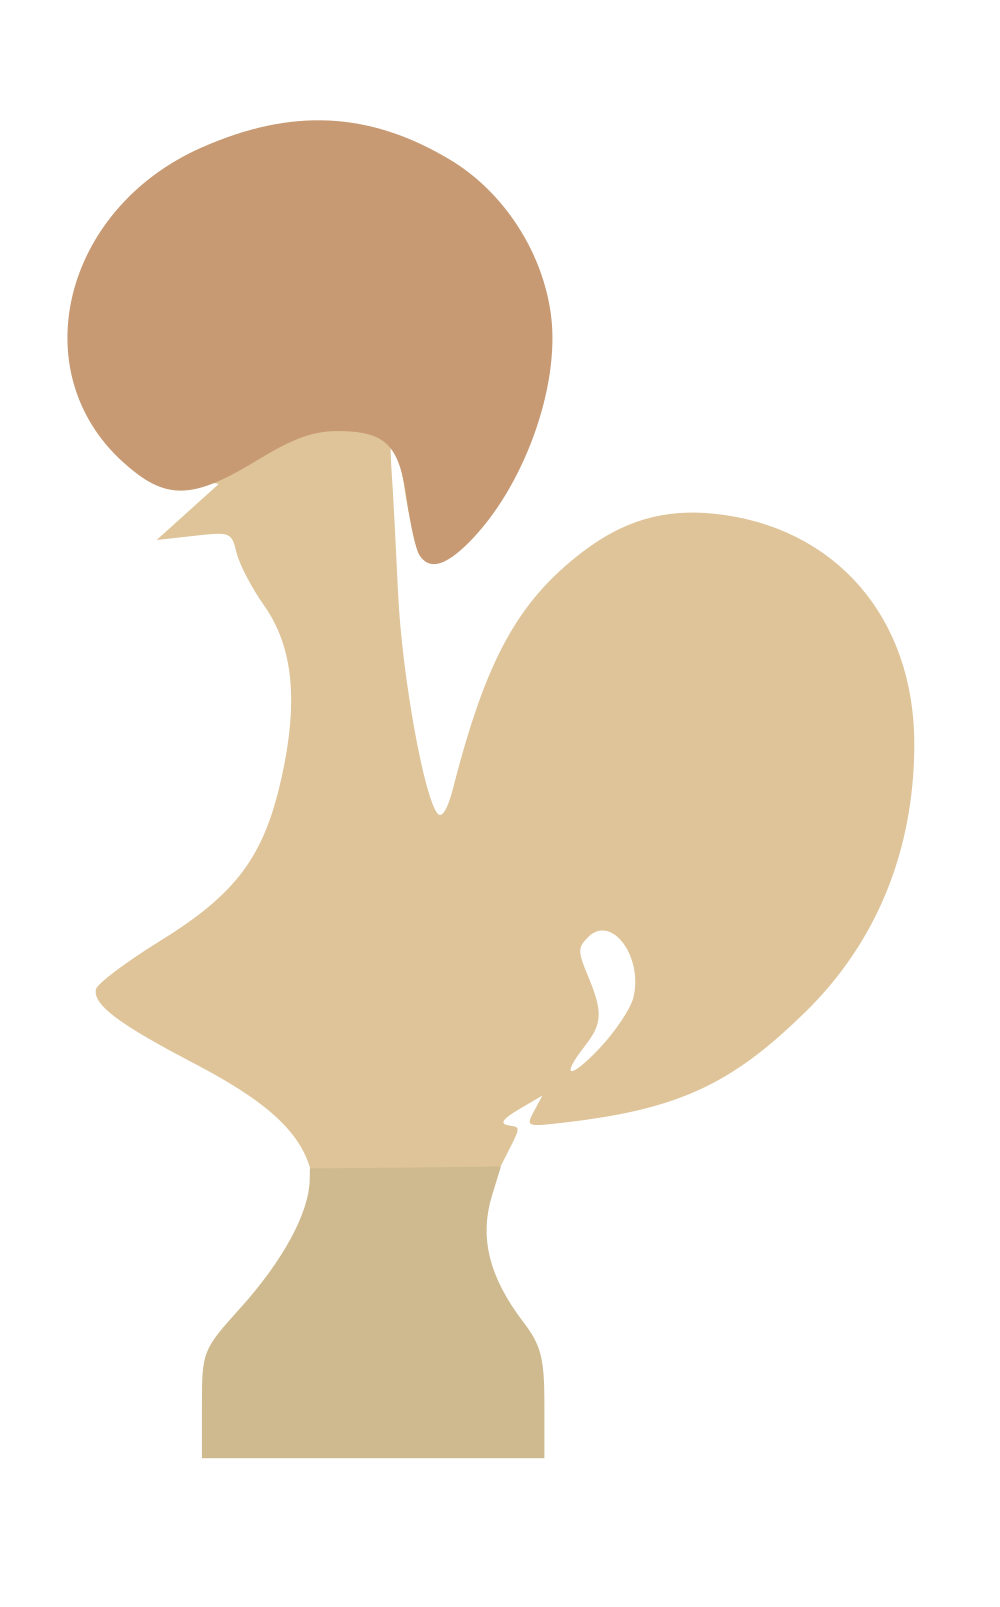
\includegraphics[width=0.15\textwidth]{coq-logo-large.png}
  \end{center}
  % go over contents of file, but skip swing tail proof, and many of the results about reachability.
\end{frame}

%%%%%%%%%%%%%%%%%%%%%%%%%%%%%%%%%%%%%%%%%%%%%%%%%%%%%%%%%%%%%%%%%%%%%%%

\end{document}
